% % % % % % % % % % % % % % % % % % % % % % % % % % % % % % % % % % % % % % % % % % % %
%                                                                                     %
% Short Sectioned Assignment LaTeX Template Version 1.0 (5/5/12)                      %
% This template has been downloaded from: http://www.LaTeXTemplates.com               %
%                                                                                     %
% Original author:  Frits Wenneker (http://www.howtotex.com)                          %
%                                                                                     %
% Modified by: Fco Javier Sueza Rodríguez (fcosueza@disroot.org)                      %
%                                                                                     %
% Changes:                                                                            %
%	    - Custom Chapters, Sections and Subsections (titlesec package)                %
%           - Document type scrbook (oneside)                                         %
%           - Use babel-lang-spanish package and marvosym                             %
%           - Use hyperref, enumitem, tcolorbox and glossaries packages               %
%           - Use Time New Roman (mathptmx), Helvetic and Courier fonts               %
%                                                                                     %
% License: CC BY-NC-SA 3.0 (http://creativecommons.org/licenses/by-nc-sa/3.0/)        %
%                                                                                     %
% % % % % % % % % % % % % % % % % % % % % % % % % % % % % % % % % % % % % % % % % % % %

%-----------------------------------------------%
%	              Packages                  %
%-----------------------------------------------%

\documentclass[paper=a4, fontsize=11pt, oneside]{scrbook}

% ---- Text Input/Output ----- %

\usepackage[T1]{fontenc}
\usepackage[utf8]{inputenc}
\usepackage{mathptmx}
\usepackage[scaled=.92]{helvet}
\usepackage{courier}
\usepackage[indent=12pt]{parskip}

\usepackage{geometry}
\geometry{verbose,tmargin=3cm,bmargin=3cm,lmargin=2.6cm,rmargin=2.6cm}

% ---- Language ----- %

\usepackage[spanish]{babel}
\usepackage{marvosym}

% ---- Another packages ---- %

\usepackage{amsmath,amsfonts,amsthm}
\usepackage{graphics,graphicx}
\usepackage{titlesec}
\usepackage{fancyhdr}
\usepackage{tcolorbox}
\usepackage{hyperref}
\usepackage{enumitem}
\usepackage[automake]{glossaries}

%--------------------------------------------------------------------%
%                      Customizing Document                          %
%--------------------------------------------------------------------%


% ----------- Custom Chapters, Sections and Subsections -------------- %

\titleformat{\chapter}[display]
			{\bfseries\Huge}
			{Tema \ \thechapter} {0.5ex}
			{\vspace{1ex}\centering}

\titleformat{\section}[hang]
			{\bfseries\Large}
			{\thesection}{0.5em}{}

\titleformat{\subsection}[hang]
			{\bfseries\large}
			{\thesubsection}{0.5em}{}

\titleformat{\subsubsection}[hang]
			{\bfseries\large}
			{\thesubsubsection}{0.5em}{}

\hypersetup{
    colorlinks=true,
    linkcolor=black,
    urlcolor=magenta
}

% ------------------- Custom heaaders and footers ------------------- %

\pagestyle{fancyplain}

\fancyhead[]{}
\fancyfoot[L]{}
\fancyfoot[C]{}
\fancyfoot[R]{\thepage}

\renewcommand{\headrulewidth}{0pt} % Remove header underlines
\renewcommand{\footrulewidth}{0pt} % Remove footer underlines

\setlength{\headheight}{13.6pt} % Customize the height of the header

% --------- Numbering equations, figures and tables ----------------- %

\numberwithin{equation}{section} % Number equations within sections
\numberwithin{figure}{section} % Number figures within sections
\numberwithin{table}{section} % Number tables within sections

% ------------------------ New Commands ----------------------------- %

\newcommand{\horrule}[1]{\rule{\linewidth}{#1}} % Create horizontal rule command


%----------------------------------------------------------------------------------------
%	TÍTULO Y DATOS DEL ALUMNO
%----------------------------------------------------------------------------------------

\title{
\vspace{10ex}
\normalfont \normalsize
\huge \textbf{Actividades de la Unidad 3: La Seguridad Social}
}
\author{Francisco Javier Sueza Rodríguez}
\date{\normalsize\today}

%----------------------------------------------------------------------------------------
%                                     DOCUMENTO
%----------------------------------------------------------------------------------------
\begin{document}

\maketitle

\thispagestyle{empty}

\vspace{75ex}

\begin{center}
    \begin{tabular}{l l}
        \textbf{Centro}: & IES Aguadulce \\
        \textbf{Ciclo Formativo}: & Desarrollo Aplicaciones Web (Distancia)\\
        \textbf{Asignatura}: & Formación y Orientación Laboral\\
        \textbf{Tema}: & Tema 3 -  La Seguridad Social\\
    \end{tabular}
\end{center}

\newpage

\tableofcontents

\newpage
\section{Caso Práctico}
Carlos explica a Blanca que como cualquier trabajador en España, debe estar afiliada a la Seguridad Social, es la forma de que participe en el sistema cotizando como trabajadora en activo y de ese modo todos los trabajadores en España, sean del sector que sean y realicen cualquier actividad económica, podamos estar cubiertos, no sólo en asistencia sanitaria, sino también en cuestiones de desempleo y protección.

\section{Enunciado}

\subsection{Actividad 1}
Una vez trabajada y visto el tema que nos ocupa, te sugiero que elijas una de estas dos opciones:

\begin{enumerate}[label=\alph*)]
    \item Aporta alguna idea o sugerencia personal que consideras que serían convenientes introducir o modificar en la Seguridad Social para mejorar el sistema y justifícala.
    \item Haz una valoración personal sobre la Seguridad Social.
\end{enumerate}

\subsection{Actividad 2}
Contesta las siguientes cuestiones que se plantean:

\begin{enumerate}[label=\alph*)]
    \item Define qué es una contingencia común y ejemplifica.
    \item Define qué es una contingencia profesional y ejemplifica.
    \item Cita los diferentes tipos de prestaciones que nos ofrece la Seguridad Social.
    \item Cita las modalidades de prestaciones de la Seguridad Social y cada modalidad ejemplifícala.
\end{enumerate}

\subsection{Actividad 3}
Cumplimenta el siguiente cuadro indicando el régimen  en el que quedan incluidos las personas que aparecen indicadas (puedes marcar con una X). Si en alguno de los ejemplos quieres añadir o comentar algo puedes hacerlo tras el cuadro.

\begin{figure}[H]
    \centering
    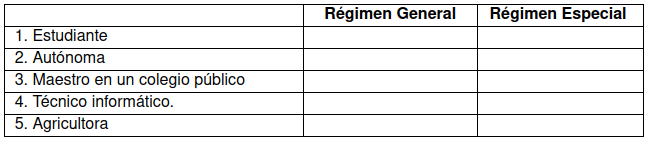
\includegraphics[scale=0.50]{tabla.png}
    \caption{Tabla a rellenar con el régimen de la SS}
\end{figure}

\subsection{Actividad 4}
Cita, señala o contesta brevemente:

\begin{enumerate}
    \item Obligaciones formales del empresario con la Seguridad Social.
    \item Sujeto responsable del pago de cuotas (patronal y obrera).
    \item Durante la huelga, ya visto en el tema anterior, ¿Qué sucederá con la obligación económica del pago a la Seguridad Social?
    \item Realiza las capturas de la página web de la Seguridad Social en el que  podemos descargar los modelos referentes al alta y baja de una persona trabajadora.
\end{enumerate}

\subsection{Actividad 5}
Teniendo en cuenta la nómina de la tarea de la unidad anterior (UT01). Determina:

\begin{enumerate}[label=\alph*)]
    \item Las bases de cotización del supuesto explicando cómo se obtienen.
    \item Las cuotas correspondientes al trabajador y el cálculo de las mismas.
    \item La cuotas correspondientes al empresariado y el cálculo de las mismas.
\end{enumerate}

Si en la tarea anterior realizaste la nómina, sólo sería calcular como novedad las deducciones aplicándoles los tipos de cotización (si es que no llegaste a calcularlo). Si tuviste algún error es momento ahora para corregirlo. Si no llegaste a realizarla, ahora puedes hacerlo.

\subsection{Actividad 6}
\begin{enumerate}[label=\alph*)]
    \item Explica los requisitos básicos y necesarios para poder acceder a una protección contributiva.
    \item Supuesto práctico:

    Todas las personas aquí expuestas creen que tienen derecho a algún tipo de prestación económica de la seguridad social en la modalidad contributiva. Indícales en principio cuál sería y los requisitos para acceder a ella, así como la cuantía, duración y aspectos más relevantes.

    \begin{enumerate}
        \item María José está actualmente embarazada de 7 meses y ya no está en condiciones de trabajar por el ritmo que implica su trabajo. Está  afiliada, dada de alta y trabajando en su empresa desde hace 5 años. Su edad es de 35 años.de baja por maternidad  está afiliada y en alta
        \item Marta, ante la incertidumbre que tiene en su empresa, ha decidido acogerse a una excedencia voluntaria para prepararse unas oposiciones al cuerpo de bomberos.
        \item Ángel, está de baja por una gripe y lleva tres años trabajando en una empresa dado de alta.
        \item Manuel necesita saber para el año 2023 en qué momento nos encontramos del sistema transitorio de pensiones.
    \end{enumerate}
\end{enumerate}

\subsection{Actividad 7}
En estos supuestos prácticos identifica, justifica y expón las posibles situaciones legales de desempleo.

\begin{enumerate}
    \item Pablo ha sido despedido por la empresa aplicándole un despido disciplinario calificado por el juez como procedente
    \item Silvia estando en periodo de prueba ha renunciado voluntariamente en su nueva empresa pero en la anterior estuvo siete años cotizando.
    \item Miriam empresaria ha rescindido  en periodo de prueba el contrato a Bernabé. Tiene acumulado de paro en los últimos seis años 359 días.
\end{enumerate}

\subsection{Actividad 8}
Oscar se queda en paro en el mes de mayo. Su Base de Cotización de los últimos seis meses ha sido de 1800 € mensuales, y ha cotizado 1240 días en los últimos seis años.

\begin{enumerate}
    \item Calcula la prestación de desempleo a la que tiene derecho y expón el procedimiento seguido para obtenerla.
    \item Haz una captura de la entidad que gestiona dicha prestación.
    \item Cita los requisitos para tener derecho al cobro de la prestación en la modalidad contributiva.
\end{enumerate}

\section{Solución}

\subsection{Actividad 1}
En nuestro caso, hemos elegido la \textbf{opción a} y vamos a aportar alguna idea que sería conveniente introducir en la Seguridad Social.




% Bibliography

\newpage
\bibliography{citas}
\bibliographystyle{unsrt}

\end{document}